\documentclass[a4paper,12pt,exos]{nsi} 
\usepackage{mathtools}
\usepackage{hyperref}



\pagestyle{empty}

\begin{document}
    \classe{\premiere spe}
    \titre{DL - Le champ de pissenlits}
    \maketitle


\dleft{13cm}{
    Le gazon d'un champ de 5000 m$^2$ est envahi par des pissenlits qui détruisent 20 \% de la surface en un an.\\
Chaque automne, Catherine arrache 250 m$^2$ de pissenlits afin de semer de la pelouse.
}
{
    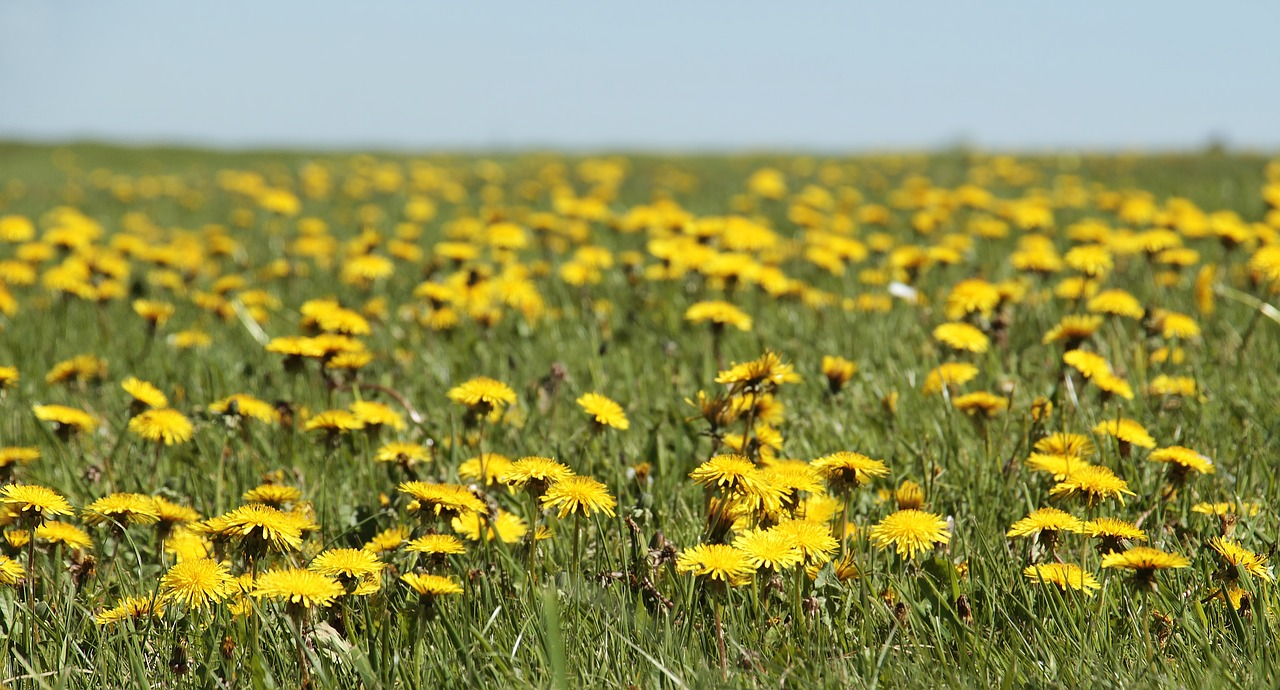
\includegraphics[width=3.5cm]{dandelion.jpg}

    \tiny{Crédits : NoName13 / Pixabay}
}

Modéliser cette situation et répondre aux questions suivantes :
\begin{enumerate}[label=\textbullet]
    \item Quelle surface de pelouse restera-t-il au bout d'un an ? de deux ans ? de 5 ans ?
    \item Quelle semble être l'évolution de la surface de pelouse au cours du temps ?
    \item La surface de pelouse pourra-elle inférieure à 2000 m$^2$ ? inférieure à 1000 m$^2$ ? Si oui, au bout de combien d'années ?
\end{enumerate}

Présenter à l’oral durant 2 minutes maximum la situation, la modélisation et les réponses aux questions posées.\\

\dleft{13.5cm}{
        
        Critères d'évaluation : 
        \begin{enumerate}[label=\textbullet]
            \item Qualité de la parole ;
            \item Qualité du discours ;
            \item Connaissances mathématiques.
        \end{enumerate}
        \textit{Lien pour l'enregistrement :} \href{www.mon-oral.net/a/MDCXNGZ2}{www.mon-oral.net/a/MDCXNGZ2}
    }
    {
\includegraphics[width=3cm]{code-qr.png}}


\end{document}